\begin{note}
    Производная не может иметь разрывов I рода.\\
    При помощи теоремы Лагранжа можно доказать, что если функция дифференцируема на $(c, c+\delta)$, где $\delta > 0$, то 
    \[f_+'(c) = \lim_{x \to c+0} f'(x)\]
    На это равенство и была дана \hyperlink{task1}{эта задача}.
    Для прочей ясности приведу план решения этой задачи: Так как функция дифференцируема на $(c, c+\delta)$, то она и непрерывна на $(c, c+\delta)$.
    Зафиксируем любое $x$ из интервала $(c, c+\delta)$, тогда по \hyperlink{lagrange}{теореме Лагранжа} $\exists \ \theta$, такое что \[f'(\theta) = \frac{f(x)-f(c)}{x-c}\]
    Теперь перейдем к пределу в равенстве $x \to c+0$, тогда $\theta \to c+0$ (то есть левая часть равна $f'(c+0)$), а предел правой не что иное, как $f_+'(c)$, получаем требуемое равенство.\\
    \textit{Фрагмент выше не является частью конспекта лекции и создан лишь для прояснения замечания ниже}.

    Так как $f_-'(a) = f'(a) = f_+'(a)$ и из \hyperlink{task1}{задачи} $f'(a-0) = f_-'(a)$, $f_+'(a) = f'(a+0)$, то $f'(a-0) = f_-'(a) = f'(a) = f_+'(a) = f'(a+0) \Rightarrow f'(a-0) = f'(a+0) = f'(a)$, то есть разрыва I рода быть не может.
\end{note}

\begin{example}
    Разрыв II рода может существовать.\\
    \[f(x) = \begin{cases}
        x^2\sin\frac{1}{x}, \quad x \neq 0\\
        0, \quad x = 0
    \end{cases}\]
    $x \neq 0: f'(x) = 2x\sin\frac{1}{x}-\cos\frac{1}{x}$\\
    $x = 0: f'(0) = \frac{f(x)-f(0)}{x-0} = \lim_{x \to 0} x\sin{\frac{1}{x}} = 0$\\
    $f'$ определена везде, но $\nexists f'(\pm 0)$.
\end{example}

\begin{theorem}
    (Дарбу)\\
    Если $f$ дифференцируема на $[a, b]$ и число $s$ лежит между $f'(a)$ и $f'(b)$,
    то найдется точка $c \in [a, b]$, такая что $f'(c) = s$.
\end{theorem}

\begin{proof}
    Если $s$ совпадает с $f'(a)$ или $f'(b)$, то условие очевидно.
    Пусть для определенности $f'(a) < s < f'(b)$.
    Рассмотрим $\phi(x) = f(x) - s \cdot x$, тогда $\phi$ дифференцируема на $[a, b]$
    и $\phi'(a) = f'(a) - s < 0 < f'(b) - s = \phi'(b)$.
    По теореме Вейерштрасса $\exists c \in [a, b] : \phi(c) = inf_{[a, b]}\phi(x)$. Если $c = a$, то
    $\frac{\phi(x)-\phi(a)}{x-a} \geq 0$ на $[a, b] \Rightarrow \phi'(a) = \phi_+'(a) = \lim_{x \to a+0} \frac{\phi(x)-\phi(a)}{x-a} \geq 0$!!! (пришли к противоречию с $\phi'(a) < 0$).
    Следовательно, $c != a$. Аналогично, $c != b$. Поэтому $c \in (a, b)$ по теореме Ферма $\phi'(c) = 0 \iff f'(c) = s$.
\end{proof}

\subsection{Приложение теорем о среднем}
Среди многочисленных приложений \hyperlink{lagrange}{теоремы Лагранжа} выделяют следующие:\\
\begin{theorem}\hypertarget{th10}{(условие монотонности)}\\
    Пусть $f$ непрерывна на промежутке $I$ и дифференцируема на $int(I)$, тогда
    \begin{enumerate}
        \item Функция нестрого возрастает (убывает) на $I$ $\iff f'(x) \geq 0 \ \ \forall x \in int(I)$.
        \item Если $f'(x) > 0 \ \ \forall x \in int(I)$, то $f(x)$ строго возрастает на I.
        \item $f$ постоянна на $I$ $\iff f'(x) = 0 \ \ \forall x \in int(I)$.
    \end{enumerate}
\end{theorem}

\begin{proof} \ \\
    (1.$\Rightarrow$) Пусть $f$ нестрого возрастает на $I$, $x \in int(I)$.
    Тогда $f(y) \geq f(x) \ \ \forall y \in (x, supI)$, и значит, $f'(x) = \lim_{y \to x+0} \frac{f(y)-f(x)}{y-x} \geq 0$.\\
    (1.$\Leftarrow$) Пусть $X, Y \in I$, x < y. Тогда по \hyperlink{lagrange}{теореме Лагранжа} $f(y)-f(x) = f'(c)(y-x)$ для некоторой точки $c \in (x, y)$.
    Так как $c \in int(I)$, то $f'(c) \geq 0$, и значит, $f(y) \geq f(x)$, то есть $f$ нестрого возрастает на $I$.
    Доказательство для нестрого убывающей аналогично или может быть сведено к рассмотрению замены $f$ на $-f$.\\
    (2) Если $f'(x) > 0 \ \ \forall x \in int(I)$, то $f(y) > f(x)$ и $f$ строго возрастает на $I$.\\
    (3) Пункт вытекает из пункта (1).\\
    Обратное утверждение пункта (2) неверно. $f(x) = x^3$ строго возрастает на $\R$, но $f'(0) = 0$.
\end{proof}

\begin{corollary}
    (достаточность условия)\\
    Пусть $f$ определена на $(\alpha, \beta)$ и $a \in (\alpha, \beta)$.
    Пусть $f$ дифференцируема на $(\alpha, \beta) \setminus \{a\}$ и непрерывна в точке $a$.
    \begin{enumerate}
        \item Если $f' \geq 0$ на $(\alpha, a)$ и $f' \leq 0$ на $(a, \beta)$, то $a$ - точка локального максимума функции $f$.
        (строгого, если неравенство строгое).
        \item Если $f' \leq 0$ на $(\alpha, a)$ и $f' \geq 0$ на $(a, \beta)$, то $a$ - точка локального минимума функции $f$.
        (строгого, если неравенство строгое).
    \end{enumerate}
\end{corollary}

\begin{proof}
    По \hyperlink{th10}{теореме об условии монотонности} $f$ нестроого возрастает на $(\alpha, a)$ и нестрого убывает на $(a, \beta)$. Следовательно, $f(x) \leq f(a) \ \ \forall x \in (\alpha, \beta)$, то есть $a$ - точка локального максимума.
    Если неравенства строгие, то возрастаение (убывание) строгое, и значит, $f(x) < f(a) \ \ \forall x \in (\alpha, \beta) \setminus \{a\}$.
\end{proof}

\begin{note}
    Функция \[f(x) = \begin{cases}
        x^2(2 + \sin \frac{1}{x}), \quad x \neq 0 \\
        0, \quad x = 0
    \end{cases}\]
    имеет строгие минимум, однако не удовлетворяет предыдущему следствию.\\
    \begin{center}
        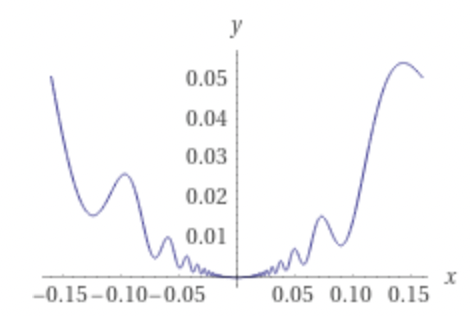
\includegraphics[width=0.55\textwidth]{x2_na_sin_1_div_x.png}
    \end{center}
\end{note}

\begin{corollary}
    (о доказательстве в неравенстве)\\
    Пусть $f, g$ непрерывны на $[a, b]$, дифференцируемы на $(a, b), \ f(a) \leq g(a)$ и $f'(x) \leq g'(x) \ \forall x \in (a, b)$.
    Тогда $f(x) \leq g(x) \ \forall x \in (a, b)$.\\
    Пусть $f, g$ непрерывны на $[a, b]$, дифференцируемы на $(a, b), \ f(a) < g(a)$ и $f'(x) < g'(x) \ \forall x \in (a, b)$.
    Тогда $f(x) < g(x) \ \forall x \in (a, b)$. 
\end{corollary}

\begin{proof}
    $h(x) = f(x) - g(x)$ непрерывна на $[a, b]$, дифференцируема на $(a, b)$, $h(a) \geq 0$, $h'(x) \underset{(<)}{\leq} 0 \ \forall x \in (a, b)$.
    По \hyperlink{th10}{теореме об условии монотонности} $h$ нестрого (строго) возрастает на $[a, b]$. 
    Поэтому $h(x) \underset{(>)}{\geq} h(a) \underset{(>)}{\geq} 0 \ \forall x \in (a, b)$.
\end{proof}

\begin{example}
    \[x-\frac{x^3}{6} < \sin x < x \ \forall x > 0\]
    Правая часть:\\
    а) при $x > 1$ очевидно \\
    б) $0 < x \leq 1, \ f(x) = \sin x, \ g(x) = x \Rightarrow f'(x) = \cos x < 1 = g'(x)$ \\
    Левая часть: \\
    $1-\frac{x^2}{2} < \cos x$\\
    Еще раз дифференцируем:
    $-x < -\sin x$\\
\end{example}

\begin{problem}
    Если $f$ непрерывна на $[a, b]$, $A$ - не более, чем счетное множество в $[a, b]$.
    Если $f$ дифференцируема на $[a, b] \setminus A$ и $f' > 0$ на $[a, b] \setminus A$, то $f$ монотонно возрастает на $[a, b]$.
\end{problem}

Важным приложением теоремы Коши о среднем является правило Лопиталя о раскрытии неопределенности.

\begin{theorem}\hypertarget{zero_on_zero_th}{(о неопределенности $\frac{0}{0}$)}\\
    Пусть $-\infty < a < b \leq +\infty$. Если
    \begin{enumerate}
        \item $f, g$ дифференцируемы на $(a, b)$.
        \item $\lim_{x \to a+0} f(x) = \lim_{x \to a+0} g(x) = 0$
        \item $g'(x) \neq 0$ на $(a, b)$
        \item $\exists \lim_{x \to a+0} \frac{f'(x)}{g'(x)} \in \overline{\R}$
    \end{enumerate}
    Тогда $\exists \lim_{x \to a+0} \frac{f(x)}{g(x)} = \lim_{x \to a+0} \frac{f'(x)}{g'(x)}$.
\end{theorem}

\begin{proof}
    Доопределим функции $f, g$ в точке $a$, положив $f(a) = g(a) = 0$,
    тогда доопределенные функции будут непрервны на $[a, b)$ и по \hyperlink{koshi_o_srednem}{теореме Коши о среднем}
    для каждого $x \in (a, b)$ существует $c \in (a, x) \ (c(x))$, такое что \[\frac{f(x)}{g(x)} = \frac{f(x)-f(a)}{g(x)-g(a)} = \frac{f'(c)}{g'(c)}\]
    Так как $c(x) \to a$ при $x \to a+0$, $c(x) \neq a$, то по свойству предела композиции \[\exists \lim_{x \to a+0} \frac{f(x)}{g(x)} = \lim_{c \to a+0} \frac{f'(c)}{g'(c)}\]
\end{proof}
\begin{theorem}\hypertarget{inf_on_inf_th}{(о неопределенности $\frac{\infty}{\infty}$)}\\
    Пусть $-\infty < a < b \leq +\infty$. Если
    \begin{enumerate}
        \item $f, g$ дифференцируемы на $(a, b)$.
        \item $\lim_{x \to a+0} g(x) = \pm \infty$
        \item $g'(x) \neq 0$ на $(a, b)$
        \item $\exists \lim_{x \to a+0} \frac{f'(x)}{g'(x)} = A \in \overline{\R}$
    \end{enumerate}
    Тогда $\exists \lim_{x \to a+0} \frac{f(x)}{g(x)} = \lim_{x \to a+0} \frac{f'(x)}{g'(x)}$.
\end{theorem}

\begin{proof} \ \\
    I) A = 0\\
    Рассмотрим произвольную $\{x_n\} \subset (a, b), \ x_n \to a$.
    Покажем, что $\frac{f(x_n)}{g(x_n)} \to 0$. Зафиксируем $\epsilon > 0$.
    По условию $\exists y \in (a, b) \ : \ \ \forall c \in (a, y) \ (g(c) \neq 0$ и $|\frac{f'(c)}{g'(c)}| < \epsilon)$.
    Без ограничения общности можно счиать, что все $x_n \in (a, y)$.
    Тогда по \hyperlink{koshi_o_srednem}{теореме Коши о среднем} $\ \forall n \in \N \ \exists c_n \in (a, x_n)$
    \[\frac{f(x_n)}{g(x_n)} = \frac{f(x_n)-f(y)}{g(x_n)-g(y)} \cdot \frac{g(x_n)-g(y)}{g(x_n)} + \frac{f(y)}{g(x_n)} =\] 
    \[= \frac{f'(c_n)}{g'(c_n)}(1-\frac{g(y)}{g(x_n)}) + \frac{f(y)}{g(x_n)} \Rightarrow\]
    \[\Rightarrow \lvert\frac{f(x_n)}{g(x_n)}\rvert \leq \epsilon(1+\lvert\frac{g(y)}{g(x_n)}\rvert + \lvert\frac{f(y)}{g(x_n)}\rvert \to \epsilon \ (due \  to \ g(x_n) \to \infty)\]
    Следовательно, $\overline{\lim_{n \to \infty}} \lvert\frac{f(x_n)}{g(x_n)}\rvert \leq \epsilon$.
    Так как $\epsilon > 0$ - любое, то $\overline{\lim_{n \to \infty}} |\frac{f(x_n)}{g(x_n)}| = 0$,
    тогда $\underline{\lim_{n \to \infty}} |\frac{f(x_n)}{g(x_n)}| \leq \overline{\lim_{n \to \infty}} |\frac{f(x_n)}{g(x_n)}| = 0$,
    и значит, $\exists \lim_{n \to \infty} \frac{f(x_n)}{g(x_n)} = 0$.\\
    II) Пусть $A \in \R$ - произвольное число. Рассмотрим $h = f - Ag$.
    Тогда \[\lim_{x \to a+0} \frac{h'(x)}{g'(x)} = \lim_{x \to a+0} (\frac{f'(x)}{g'(x)} - A) = 0\]
    Поэтому по пункту (I) $\exists \lim_{x\to a+0} \frac{h(x)}{g(x)} = 0$, то есть $\lim_{x\to a+0} \frac{f(x)}{g(x)} = A$.\\
    III) $A = +\infty$. Аналогично пункту I зафиксируем $M > 0$, что $\frac{f'(c)}{g'(c)} > M$.
    Тогда \[\frac{f(x_n)}{g(x_n)} = \frac{f'(c_n)}{g'(c_n)}(1-\frac{g(y)}{g(x_n)}) + \frac{f(y)}{g(x_n)}\]
    Пусть $(1-\frac{g(y)}{g(x_n)}) > 0$ при $n \geq n_0$.
    \[\frac{f(x_n)}{g(x_n)} \geq M(1-\frac{g(y)}{g(x_n)}) + \frac{f(y)}{g(x_n)} \to M\]
    Следовательно, $\underline{\lim_{n \to \infty}} |\frac{f(x_n)}{g(x_n)}| \geq M$.
    Так как $M > 0$ - любое, то \[\underline{\lim_{n \to \infty}} \frac{f(x_n)}{g(x_n)} = +\infty\ \Rightarrow \lim_{n \to \infty} \frac{f(x_n)}{g(x_n)} = +\infty\]
\end{proof}